\section{Реализация на началния екран на приложението}
Началният екран на мобилното приложение съдържа в себе си галерия с всичкимебели, които се предлагат. Всяка мебел се дефинира от 5 качества, а именно:
\begin{itemize}
    \item \textbf{name}\par
    Низ от символи, който определя името на предлагания продукт.

    \item \textbf{price}\par
    Низ от символи, който определя името на цената продукт.

    \item \textbf{imagePath}\par
    Низ от символи, който определя локацията, на която снимка на мебелта може да бъде достъпена. Тази локация може да е локална, на устройството на потребителя или глобална, в интернет мрежата.

    \item \textbf{modelPath}\par
    Низ от символи, който определя локацията, на която 3D модела може да бъде достъпен. Тази локация може да е локална, на устройството на потребителя или глобална, в интернет мрежата.

    \item \textbf{isLocal}\par
    Булева променива, която определя дали изображението и 3D модела на предмета се намират локално на устройството или в мрежата.
\end{itemize}

Тези качества са структорирани в JSON файл. Примерно, ако трябва да се съхрани конфигурация, съдържаща в себе си 3 предмета (стол, маса и хладилник), структората на JSON документа би изглеждала така:
\lstinputlisting[language=Java]{code/products.json}

В кода на приложението е дефиниран клас за подобни продукти - ProductModel, който съдържа в себе си обработената информация от JSON файла. Важно е да се отбележи, че пътя към снимката на предмета е заменен с обект съдържащ самата снимка. Същото се отнася и за 3D модела на мебелта, която по-късно ще се визуализира. Променивата \emph{isLocal} не се съхранява, но се изпозва при създаването на обектите на изображението и 3D модела:
\lstinputlisting[language=Java, linerange={6-17}]{code/product-model.dart}

В приложението, също така, е дефиниран метод, който да итерира през JSON списаци с мебели и да ги конвертира към ProductModel обекти:
\lstinputlisting[language=Java, linerange={10-16}]{code/product-list.dart}

За целта се използва метода на ProductModel - fromMapList, който получава списък от карти, съдържащи в себе си двойки ключ-стойност (на англ. ``key-value pairs''). Този списък представлява зареденият JSON файл. В метода се създава нов списък, получения като аргумент списък се обхожда, като на всеки елемент се извиква метода \emph{ProductModel.fromMap} и резултата се запазва в новия списък:
\lstinputlisting[language=Java, linerange={42-48}]{code/product-model.dart}

Статичния метод ProductModel.fromMap получава една карта, съдържащи в себе си двойки ключ-стойност и създава ProductModel обект от нея. Името и цената остават непроменени. При създаване на обекта за изображението на предмета, първо се проверява да ли то е достъпно онлайн или в локалната памет на телефона, като за целта се използва \emph{isLocal} променливата. След това се извиква съотвентния метод на вградения във Flutter клас \emph{Image}. Аналогична е ситулацията при създаване на обекта за 3D модела на предмета. Единственото нещо, което трябва да се допълни тук, че всички модели на предмети имат едно и също оразмеряване, позиция (положението на телефона) и завъртане:
\lstinputlisting[language=Java, linerange={19-40}]{code/product-model.dart}

За клиентската част на приложението се използва вградения във Flutter FutureBuilder елемент. FutureBuilder се използва за визуализиране на асинхронни данни - функцията getProduct() е асинхронна, понеже самото четене на JSON файла от локалната памет е асинхронно. Докато данните още се четат от паметта, се визуализира индикатор за зареждане; в противен случай се показва самата галерия от мебели:
\lstinputlisting[language=Java, linerange={18-41}]{code/product-list.dart}

Заредената версия на началния екран може да се наблюдава на фиг. \ref{fig:home-screen-in-3}.

\begin{figure}[H]
    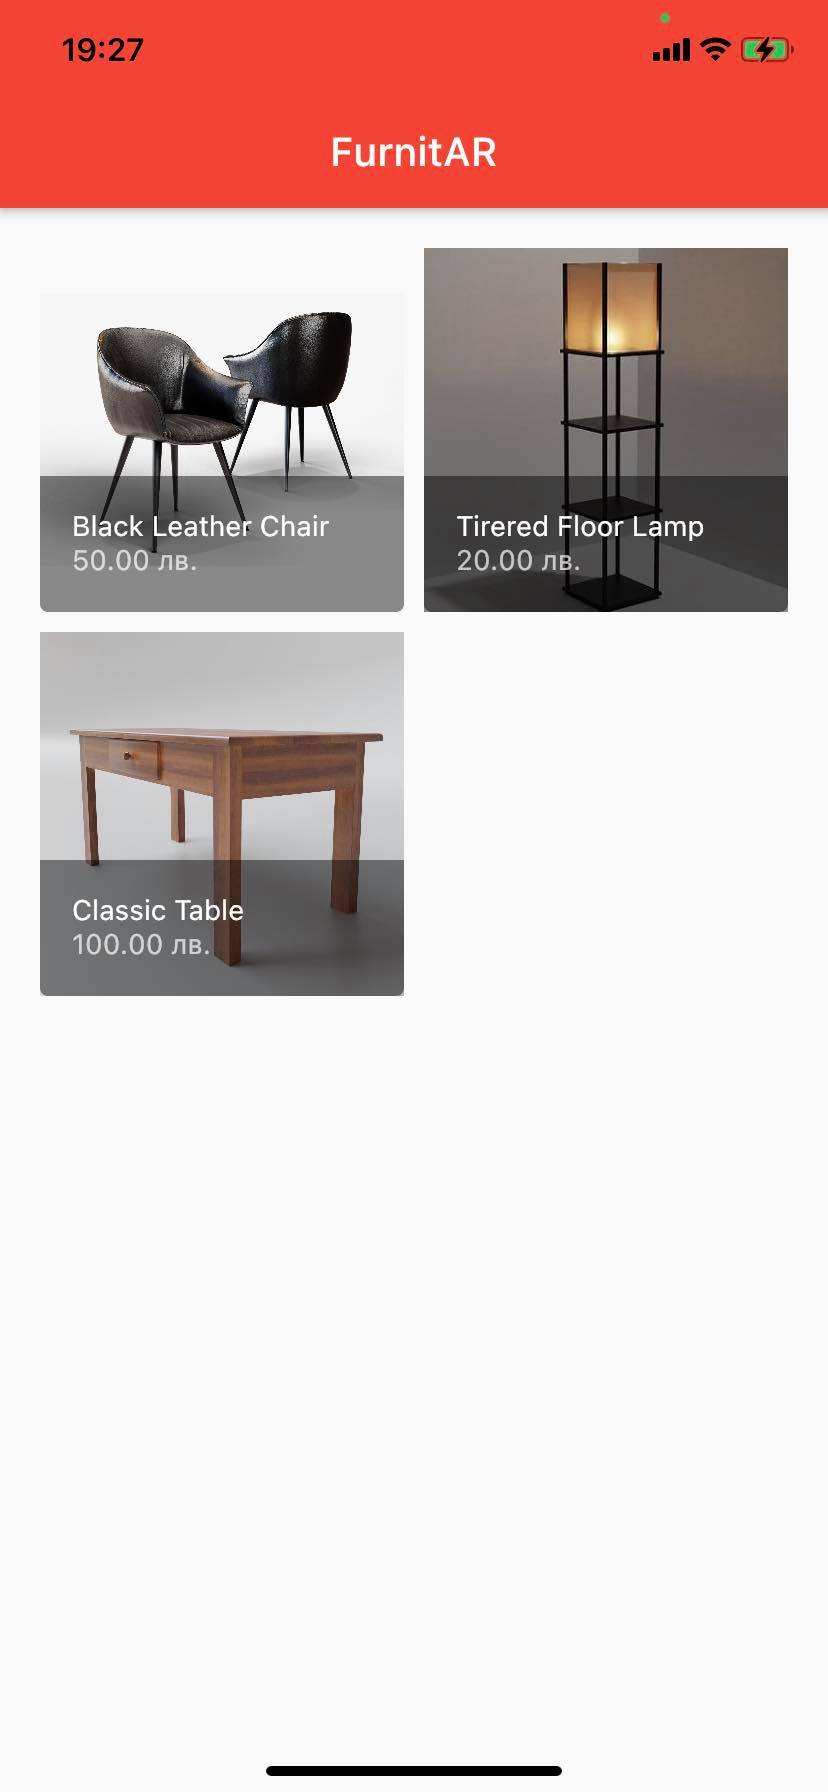
\includegraphics[width=0.4\textwidth]{home-screen-3.jpeg}
    \centering
    \caption{Начален екран на мобилното приложение}
    \label{fig:home-screen-in-3}
\end{figure}
